

\tikzset{every picture/.style={line width=0.75pt}} %set default line width to 0.75pt        

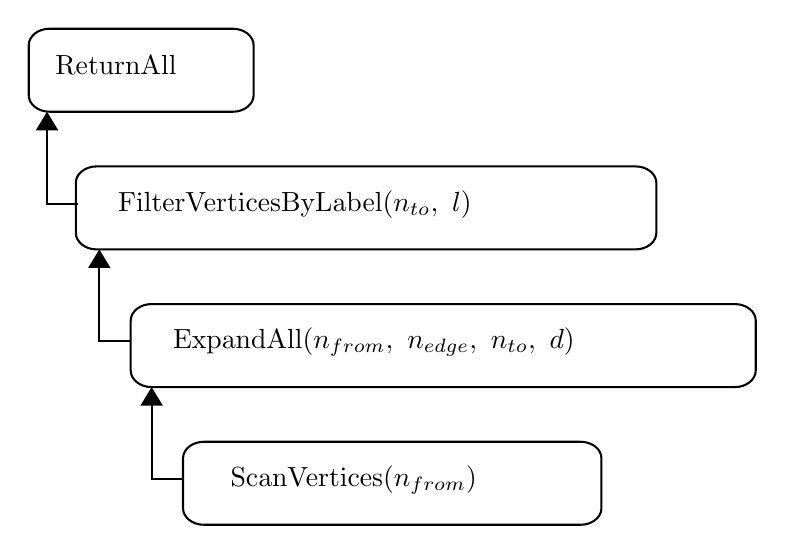
\begin{tikzpicture}[x=0.75pt,y=0.75pt,yscale=-1,xscale=1.26]
%uncomment if require: \path (0,300); %set diagram left start at 0, and has height of 300

%Rounded Rect [id:dp9370573454267987] 
\draw   (111,41) .. controls (111,36.58) and (114.58,33) .. (119,33) -- (189,33) .. controls (193.42,33) and (197,36.58) .. (197,41) -- (197,65) .. controls (197,69.42) and (193.42,73) .. (189,73) -- (119,73) .. controls (114.58,73) and (111,69.42) .. (111,65) -- cycle ;

%Rounded Rect [id:dp8665691991968861] 
\draw   (150,173.66) .. controls (150,169.24) and (153.58,165.66) .. (158,165.66) -- (381,165.66) .. controls (385.42,165.66) and (389,169.24) .. (389,173.66) -- (389,197.66) .. controls (389,202.08) and (385.42,205.66) .. (381,205.66) -- (158,205.66) .. controls (153.58,205.66) and (150,202.08) .. (150,197.66) -- cycle ;

%Rounded Rect [id:dp756749227156685] 
\draw   (170,240) .. controls (170,235.58) and (173.58,232) .. (178,232) -- (322,232) .. controls (326.42,232) and (330,235.58) .. (330,240) -- (330,264) .. controls (330,268.42) and (326.42,272) .. (322,272) -- (178,272) .. controls (173.58,272) and (170,268.42) .. (170,264) -- cycle ;

%Rounded Rect [id:dp9307818066691674] 
\draw   (129,107.33) .. controls (129,102.91) and (132.58,99.33) .. (137,99.33) -- (343,99.33) .. controls (347.42,99.33) and (351,102.91) .. (351,107.33) -- (351,131.33) .. controls (351,135.75) and (347.42,139.33) .. (343,139.33) -- (137,139.33) .. controls (132.58,139.33) and (129,135.75) .. (129,131.33) -- cycle ;

%Straight Lines [id:da678799978902756] 
\draw    (170,250) -- (158,250) -- (158,208.66) ;
\draw [shift={(158,205.66)}, rotate = 90] [fill={rgb, 255:red, 0; green, 0; blue, 0 }  ][line width=0.08]  [draw opacity=0] (8.93,-4.29) -- (0,0) -- (8.93,4.29) -- cycle    ;
%Straight Lines [id:da7443050345811884] 
\draw    (150,183.67) -- (138,183.67) -- (138,142.33) ;
\draw [shift={(138,139.33)}, rotate = 90] [fill={rgb, 255:red, 0; green, 0; blue, 0 }  ][line width=0.08]  [draw opacity=0] (8.93,-4.29) -- (0,0) -- (8.93,4.29) -- cycle    ;
%Straight Lines [id:da9837753990422333] 
\draw    (130,117.34) -- (118,117.34) -- (118,76) ;
\draw [shift={(118,73)}, rotate = 90] [fill={rgb, 255:red, 0; green, 0; blue, 0 }  ][line width=0.08]  [draw opacity=0] (8.93,-4.29) -- (0,0) -- (8.93,4.29) -- cycle    ;

% Text Node
\draw (120,44.5) node [anchor=north west][inner sep=0.75pt]   [align=left] {ReturnAll};
% Text Node
\draw (144,109.33) node [anchor=north west][inner sep=0.75pt]   [align=left] {FilterVerticesByLabel($\displaystyle n_{\text{to}} ,\ l)$};
% Text Node
\draw (165,175.66) node [anchor=north west][inner sep=0.75pt]   [align=left] {ExpandAll($\displaystyle n_{\text{from}} ,\ n_{\text{edge}} ,\ n_{\text{to}} ,\ d)$};
% Text Node
\draw (187,242) node [anchor=north west][inner sep=0.75pt]   [align=left] {ScanVertices($\displaystyle n_{\text{from}})$};


\end{tikzpicture}
